\section{Sensibilité et interprétation}
\label{sec:sensibilite}
Les analyses suivantes évaluent la sensibilité des résultats au nombre
d'initialisations, à la graine aléatoire et à la standardisation.

\subsection{Initialisation des K-means et choix d'échelle}
À graine 42 et $K=4$ constants, le TBC passe de $63{,}57\,\%$ à
$97{,}86\,\%$ entre un et 20 départs (tableau~\ref{tab:restarts}).
Aucun gain supplémentaire n'est observé entre 10, 20 et 50 départs pour cette
graine. Avec 20 départs, les graines 0 à 9 donnent encore des ARI de
$0{,}925$ à $0{,}943$ : les répétitions ne garantissent donc pas l'optimum global.

\begin{table}[H]
\centering\small
\begin{tabular}{rrrr}
\toprule
\texttt{n\_init} & ARI & TBC & Inertie ($10^6$) \\
\midrule
1 & 0{,}558 & 63{,}57\,\% & 10{,}6906 \\
10 & 0{,}943 & 97{,}86\,\% & 10{,}3462 \\
20 & 0{,}943 & 97{,}86\,\% & 10{,}3462 \\
50 & 0{,}943 & 97{,}86\,\% & 10{,}3462 \\
\bottomrule
\end{tabular}

\caption[K-means : sensibilité au nombre de départs]{Effet du nombre de départs, données réelles brutes, graine 42.}
\label{tab:restarts}
\end{table}

La standardisation ramène chaque variable à une variance unitaire
\cite{same} et change ainsi la métrique de segmentation.
Appliquée aux trois méthodes avant ajustement, elle dégrade ici leur ARI
(tableau~\ref{tab:scaling}). La première coupure Fisher passe de 35 à 21
en indices Python. Nous conservons les données brutes pour l'expérience
principale. Le déplacement de la frontière montre que les régimes détectés
dépendent de la pondération des coordonnées. Les inerties obtenues sur des
échelles différentes ne sont pas directement comparables.

\begin{table}[H]
\centering\small
\begin{tabular}{lrrr}
\toprule
Données & Fisher & K-Means (20 départs) & Ward \\
\midrule
Brutes & 1{,}000 & 0{,}943 & 0{,}859 \\
Standardisées & 0{,}781 & 0{,}735 & 0{,}545 \\
\bottomrule
\end{tabular}

\caption[ARI : sensibilité à la standardisation]{ARI à $K=4$ selon le prétraitement ; K-means à 20 départs, graine 42.}
\label{tab:scaling}
\end{table}

\begin{figure}[H]
\centering
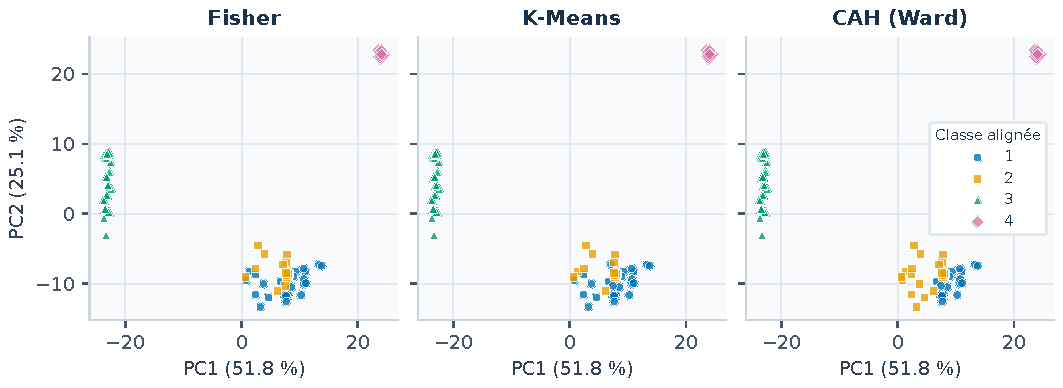
\includegraphics[width=0.98\linewidth,height=4.8cm,keepaspectratio]{aiguillage_espace.pdf}
\caption[Aiguillage : projection ACP des partitions]{Projection ACP des données centrées-réduites, colorée par les partitions
ajustées sur les variables brutes. PC1 et PC2 expliquent respectivement
\PcaOne\,\% et \PcaTwo\,\% de la variance ; les couleurs sont alignées sur la référence.}
\label{fig:acp}
\end{figure}

Dans la projection ACP (figure~\ref{fig:acp}), les classes 1 et 2 se recouvrent
davantage que les classes 3 et 4, ce qui est cohérent avec la localisation des
erreurs. Cette lecture reste partielle : environ $77\,\%$ de la variance
standardisée est représentée. Les 140 observations comprennent 128 vecteurs
distincts ; les répétitions, toutes dans la classe 3, sont conservées pour
respecter l'ordre d'acquisition.

\section{Conclusion}
Fisher distingue des régimes successifs proches dans l'espace.
La contrainte d'ordre permet ici de retrouver exactement
la partition de référence de \file{aiguillage}, tandis que les comparateurs
introduisent quelques affectations isolées entre les deux premiers régimes.
Les départs multiples des K-means réduisent nettement l'écart, et la
standardisation modifie les frontières. La pertinence de la segmentation dépend
donc à la fois de l'ordre des observations et de la métrique retenue.
